\pdfminorversion=4
\documentclass[aspectratio=169]{beamer}

\mode<presentation>
{
  \usetheme{default}
  \usecolortheme{default}
  \usefonttheme{default}
  \setbeamertemplate{navigation symbols}{}
  \setbeamertemplate{caption}[numbered]
  \setbeamertemplate{footline}[frame number]  % or "page number"
  \setbeamercolor{frametitle}{fg=white}
  \setbeamercolor{footline}{fg=black}
} 

\usepackage[english]{babel}
\usepackage[utf8x]{inputenc}
\usepackage{tikz}
\usepackage{courier}
\usepackage{array}
\usepackage{bold-extra}
\usepackage{minted}
\usepackage[thicklines]{cancel}
\usepackage{fancyvrb}

\xdefinecolor{dianablue}{rgb}{0.18,0.24,0.31}
\xdefinecolor{darkblue}{rgb}{0.1,0.1,0.7}
\xdefinecolor{darkgreen}{rgb}{0,0.5,0}
\xdefinecolor{darkgrey}{rgb}{0.35,0.35,0.35}
\xdefinecolor{darkorange}{rgb}{0.8,0.5,0}
\xdefinecolor{darkred}{rgb}{0.7,0,0}
\definecolor{darkgreen}{rgb}{0,0.6,0}
\definecolor{mauve}{rgb}{0.58,0,0.82}

\title[2020-10-01-lhcb-computing]{\only<1>{Future of}\only<2>{\xcancel{Future of} Trends in} User Analysis}
\author{Jim Pivarski}
\institute{Princeton University -- IRIS-HEP}
\date{October 1, 2020}

\usetikzlibrary{shapes.callouts}

\begin{document}

\logo{\pgfputat{\pgfxy(0.11, 7.4)}{\pgfbox[right,base]{\tikz{\filldraw[fill=dianablue, draw=none] (0 cm, 0 cm) rectangle (50 cm, 1 cm);}\mbox{\hspace{-8 cm}
\includegraphics[height=1 cm]{princeton-logo-long.png}\hspace{0.1 cm}\raisebox{0.1 cm}{
\includegraphics[height=0.8 cm]{iris-hep-logo-long.png}}\hspace{0.1 cm}}}}}

\begin{frame}
  \titlepage
\end{frame}

\logo{\pgfputat{\pgfxy(0.11, 7.4)}{\pgfbox[right,base]{\tikz{\filldraw[fill=dianablue, draw=none] (0 cm, 0 cm) rectangle (50 cm, 1 cm);}\mbox{\hspace{-8 cm}
\includegraphics[height=1 cm]{princeton-logo.png}\hspace{0.1 cm}\raisebox{0.1 cm}{
\includegraphics[height=0.8 cm]{iris-hep-logo.png}}\hspace{0.1 cm}}}}}

% Uncomment these lines for an automatically generated outline.
%\begin{frame}{Outline}
%  \tableofcontents
%\end{frame}

% START START START START START START START START START START START START START

\begin{frame}{Define: ``user analysis''}
\large
\vspace{0.65 cm}

I'm aware that LHCb is moving important physics decisions earlier in the pipeline, but I think it's still meaningful to talk about ``user analysis'' as the last step.

\begin{center}
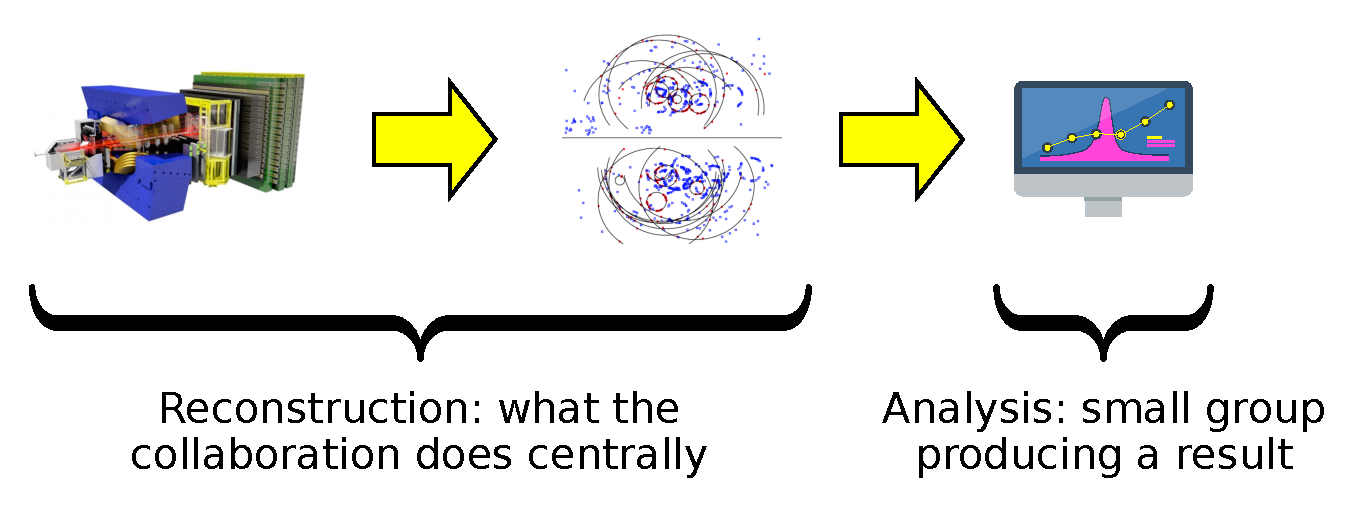
\includegraphics[width=0.9\linewidth]{img/analysis-pipeline.pdf}
\end{center}
\end{frame}

\begin{frame}{\mbox{ }}
\vspace{0.5 cm}

\begin{center}
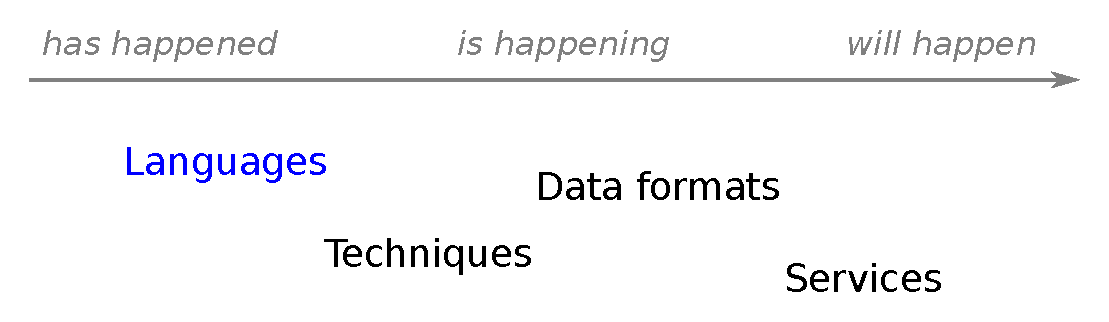
\includegraphics[width=0.9\linewidth]{img/topics-1.pdf}
\end{center}
\end{frame}

\begin{frame}{Python: the revolution has already happened}
\large
\vspace{0.5 cm}

Plot \#1: pip-install statistics in the past three years

\normalsize
\textcolor{gray}{iminuit, root-numpy, and rootpy predate the rise, and therefore set the scale.}

\begin{center}
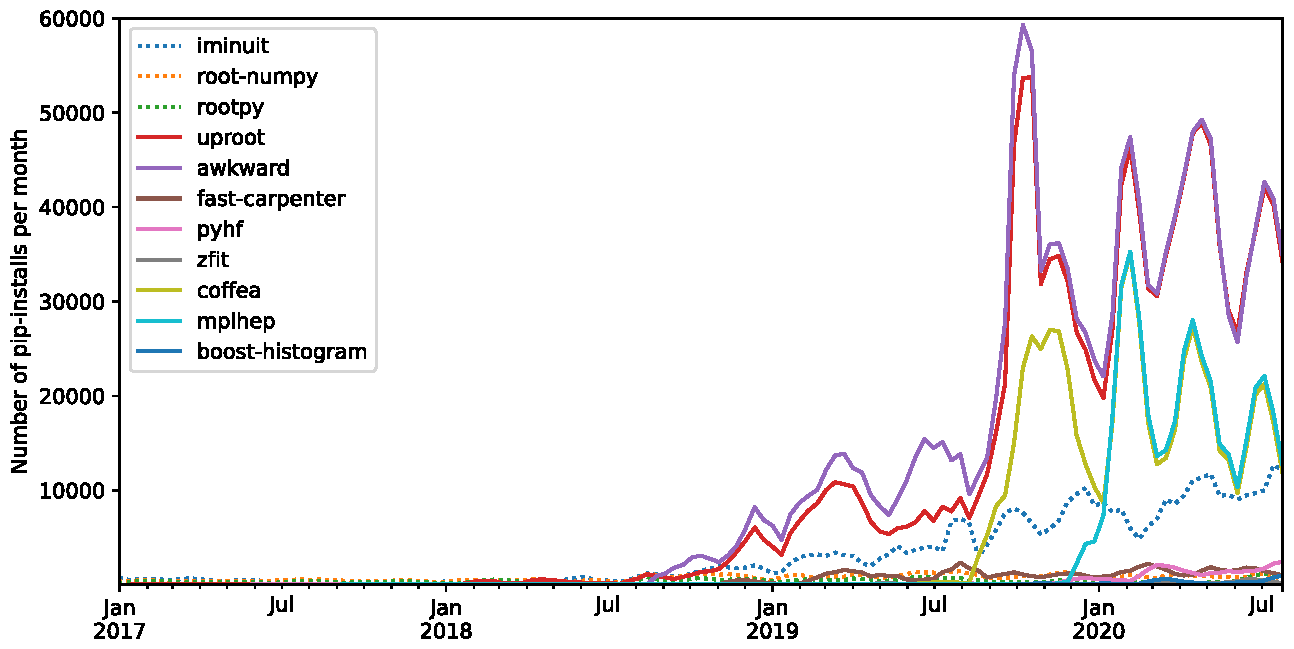
\includegraphics[width=0.85\linewidth]{img/piplinear-iminuit-rootnumpy-rootpy-uproot-awkward-fastcarpenter-pyhf-zfit-coffea-mplhep-boosthistogram.pdf}
\end{center}
\end{frame}

\begin{frame}{Python: the revolution has already happened}
\large
\vspace{0.5 cm}

Plot \#2: Language of non-fork GitHub repos by users who forked CMSSW

\normalsize
\vspace{\baselineskip}

\begin{center}
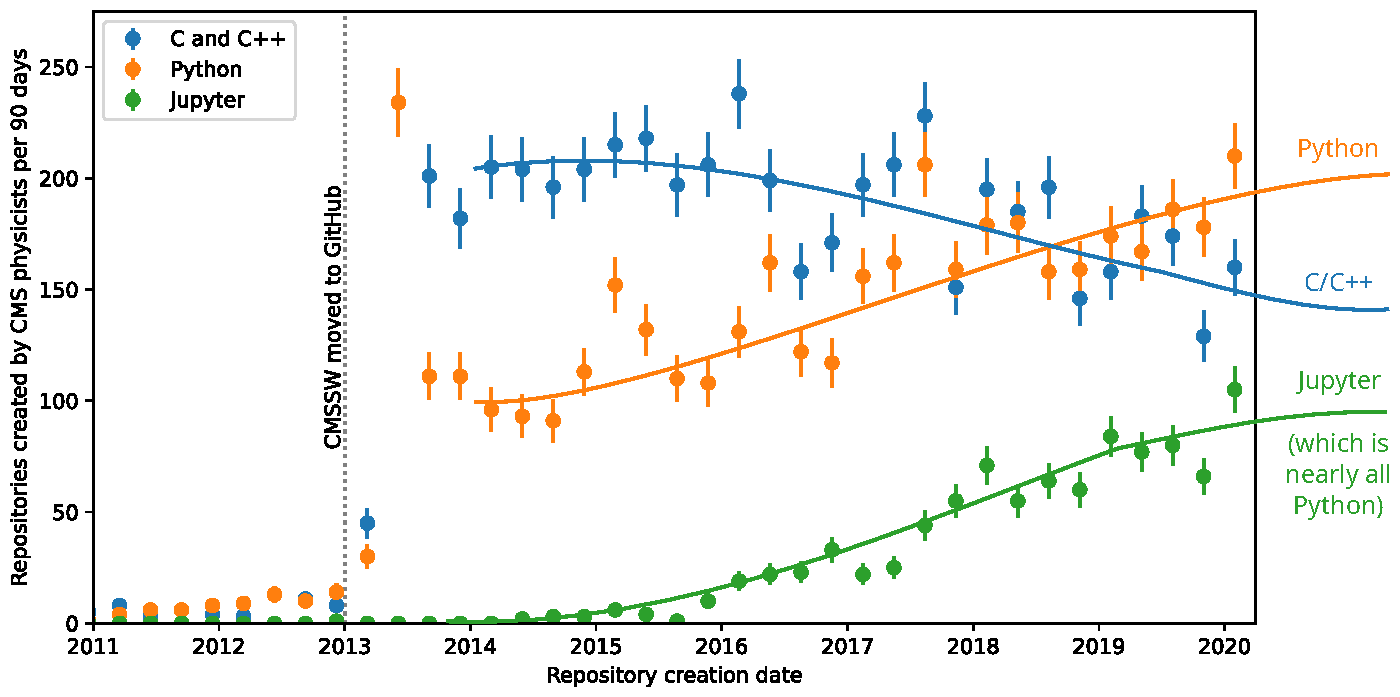
\includegraphics[width=0.85\linewidth]{img/01-github-cmssw-language.pdf}
\end{center}
\end{frame}

\begin{frame}{Python: the revolution has already happened}
\large
\vspace{0.5 cm}

Plot \#3: Search for substrings in those repos: what are those users typing?

\normalsize
\textcolor{gray}{We assume ``tfile'' correlates to ROOT; ``root'' by itself (case insensitive) is too generic.}

\begin{center}
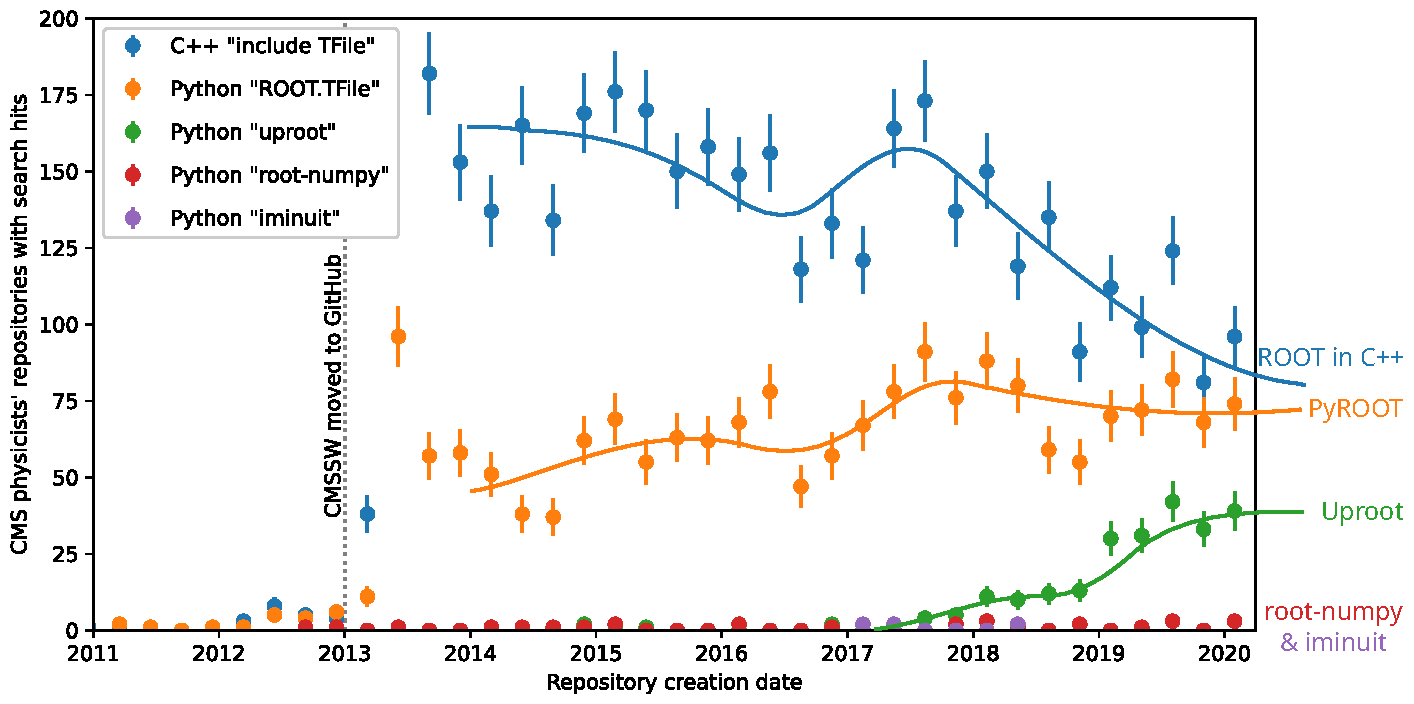
\includegraphics[width=0.85\linewidth]{img/03-github-root-python.pdf}
\end{center}
\end{frame}

\begin{frame}{Python: the revolution has already happened}
\large
\vspace{0.5 cm}

Plot \#3: What about machine learning?

\normalsize
\textcolor{gray}{{\bf Surprise:} Scikit-Learn! {\bf Not a surprise:} TMVA is the only significant C++ library.}

\begin{center}
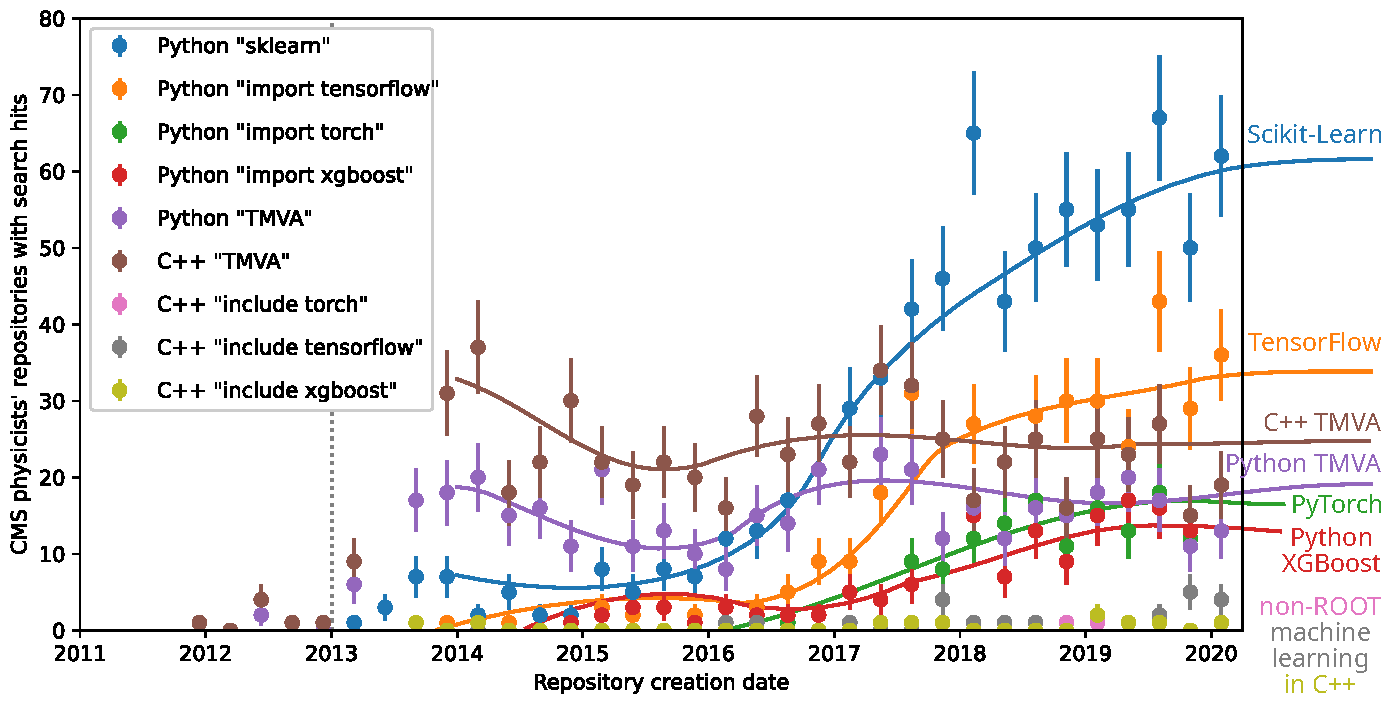
\includegraphics[width=0.85\linewidth]{img/04-github-machine-learning.pdf}
\end{center}
\end{frame}

\begin{frame}{Python: the revolution has already happened}
\large
\vspace{0.5 cm}

Plot \#4: Was Python adoption driven by Uproot or machine learning (ML)?

\normalsize
\textcolor{gray}{Twice as much basic analysis (NumPy/Matplotlib) than ML; trend predates Uproot.}

\begin{center}
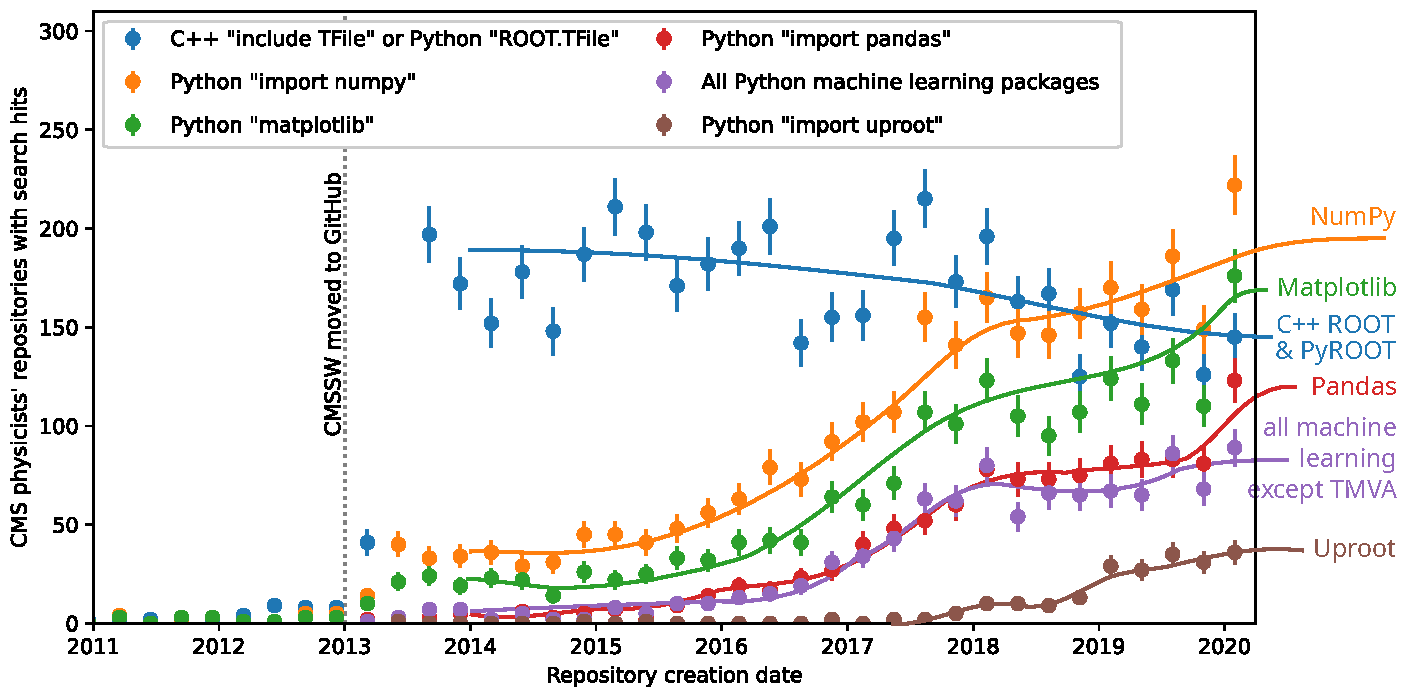
\includegraphics[width=0.85\linewidth]{img/05-github-anyroot-python-machinelearning-uproot.pdf}
\end{center}
\end{frame}

\begin{frame}{Our community doesn't change or add languages often}
\large
\vspace{0.25 cm}

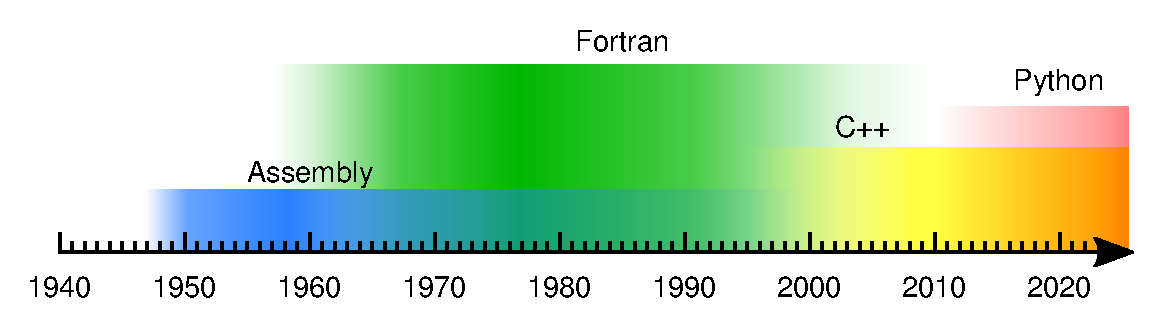
\includegraphics[width=\linewidth]{img/programming-languages.pdf}

\vspace{0.5 cm}
C++ first appeared in 1985: 10--15~years before we adopted it

\vspace{0.25 cm}
Python first appeared in 1990: 20--25~years before we adopted it

\vspace{0.25 cm}
\uncover<2->{Julia first appeared in 2012: maybe we'll be using it by 2030}
\end{frame}

\begin{frame}{An aside on future languages}
\vspace{0.5 cm}
\begin{columns}
\column{0.5\linewidth}
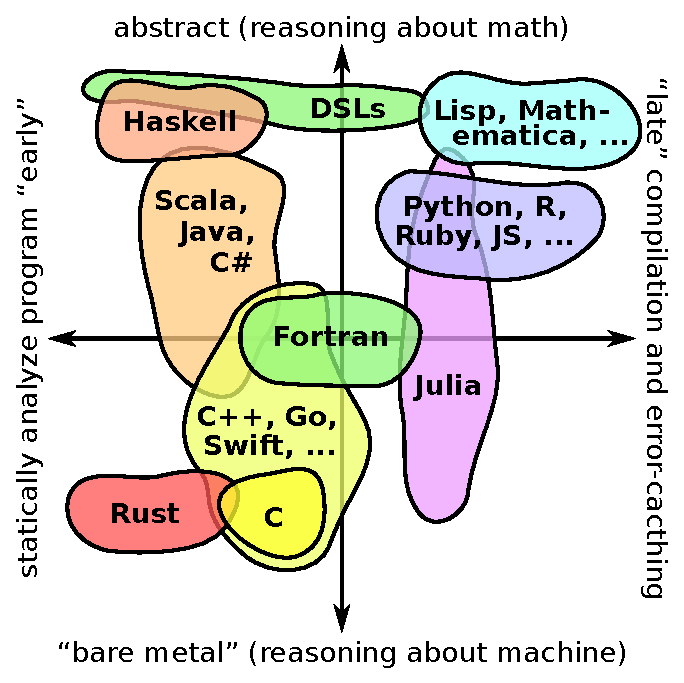
\includegraphics[width=\linewidth]{img/language-properties-grid.pdf}

\column{0.5\linewidth}
\begin{itemize}
\item \textcolor{darkblue}{Python, R, Ruby, Javascript, Lua, etc.} are all relatively abstract, late error-catching glue languages. \\ \uncover<2->{\textcolor{darkblue}{Python isn't special:} it's just where the best libraries self-gravitated.}

\item<3-> \textcolor{darkblue}{Julia} is different: everything is ``just-in-time'' (JIT) compiled, so it is flexible like Python, but fast, too.

\item<4-> \textcolor{darkblue}{Rust} is a unique extreme. Triggers?

\item<5-> \textcolor{darkblue}{DSLs (domain specific languages)} have physics concepts baked in with opportunities for strict error checking and flexible backends.

\end{itemize}
\end{columns}
\end{frame}

\begin{frame}{Some DSLs\ldots\ (see Sezen Sekmen @ LHCP 2020)}
\vspace{0.25 cm}
\begin{center}
\begin{onlyenv}<1>
\vspace{-0.25 cm}
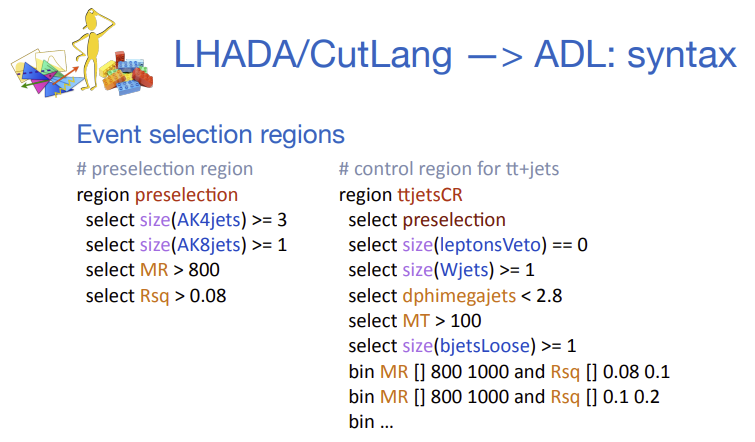
\includegraphics[width=0.8\linewidth]{img/adl-1.png}
\end{onlyenv}
\begin{onlyenv}<2>
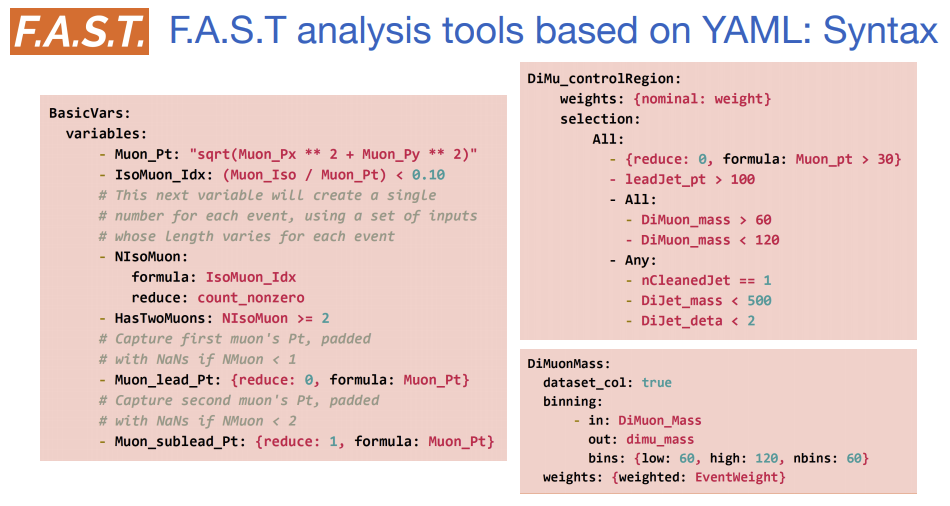
\includegraphics[width=0.9\linewidth]{img/adl-2.png}
\end{onlyenv}
\begin{onlyenv}<3>
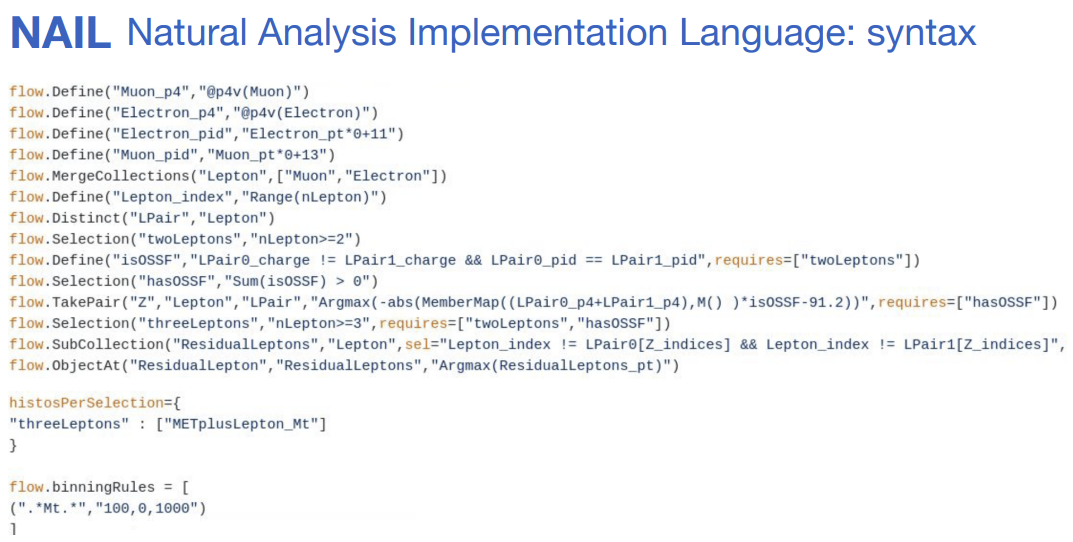
\includegraphics[width=1.0\linewidth]{img/adl-3.png}
\end{onlyenv}
\begin{onlyenv}<4>
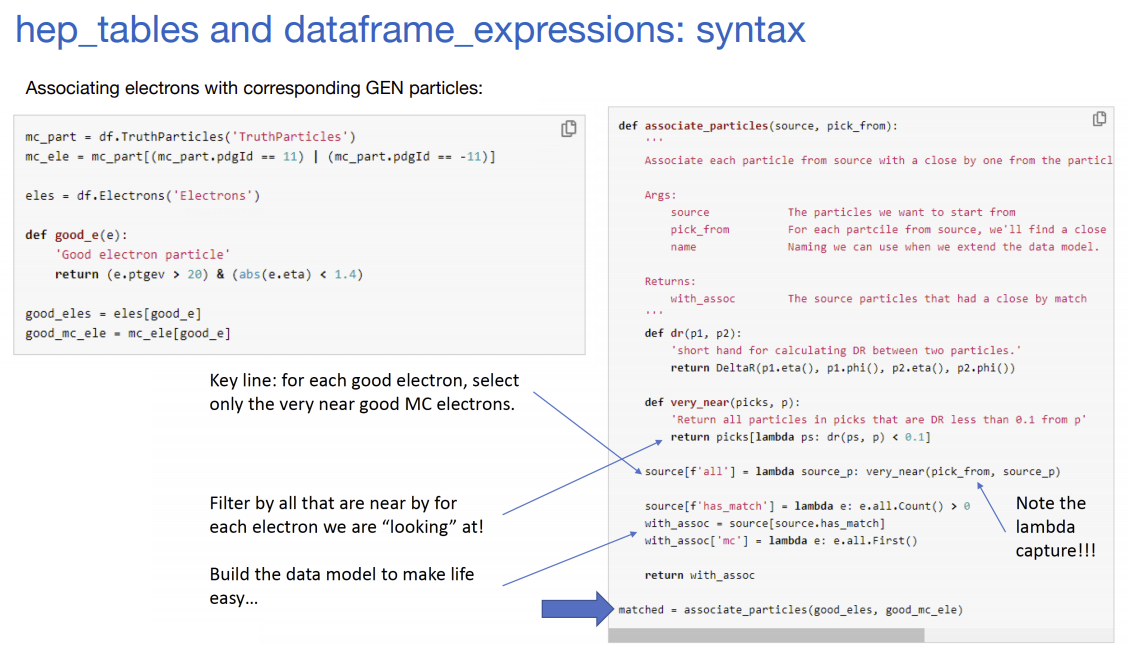
\includegraphics[width=0.9\linewidth]{img/adl-4.png}
\end{onlyenv}
\begin{onlyenv}<5>
\textcolor{darkblue}{\large PartiQL (demo) $\to$ AwkwardQL (real implementation)\hspace{3 cm}}

\vspace{0.25 cm}
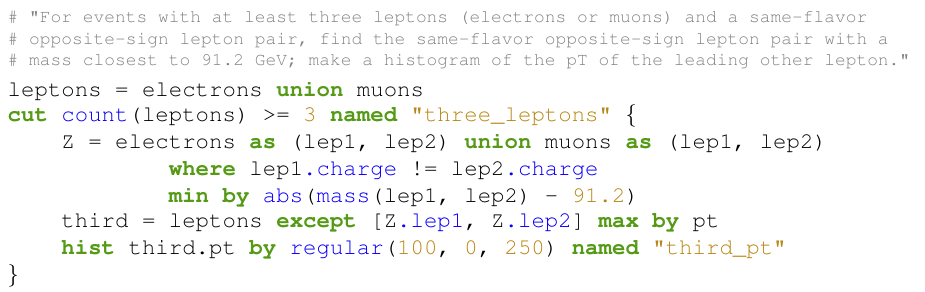
\includegraphics[width=0.9\linewidth]{img/adl-5.png}
\end{onlyenv}
\end{center}
\end{frame}

\begin{frame}{\mbox{ }}
\vspace{0.5 cm}

\begin{center}
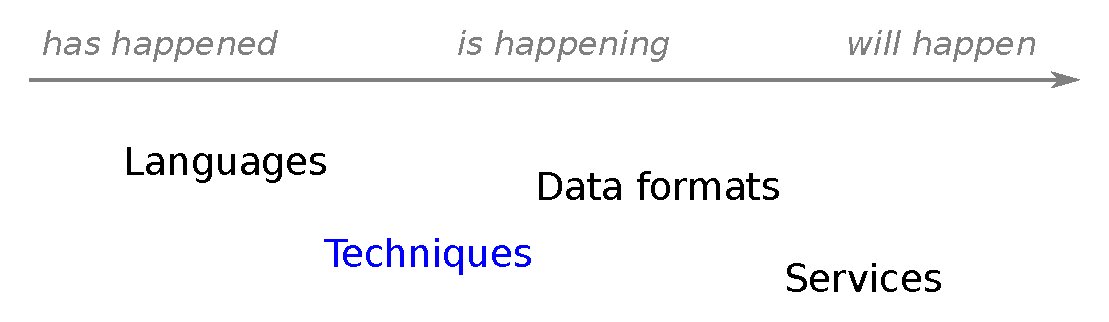
\includegraphics[width=0.9\linewidth]{img/topics-2.pdf}
\end{center}
\end{frame}

\begin{frame}[fragile]{Language choice does not determine performance!}
\vspace{0.25 cm}
\hfill\mbox{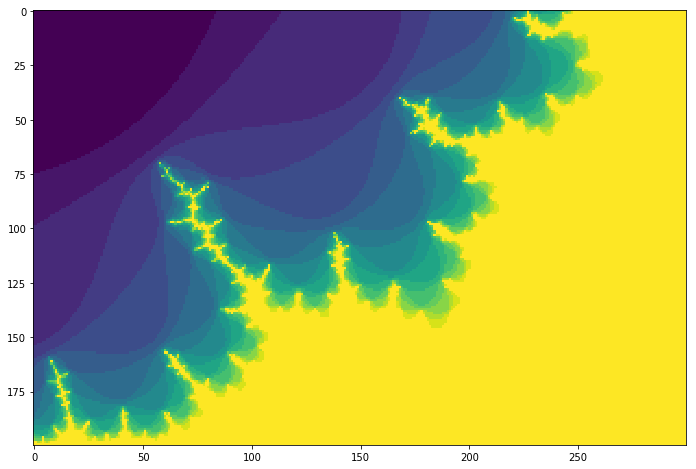
\includegraphics[height=3 cm]{img/performance-test-fractal.png}\hspace{-0.25 cm}}

\vspace{-2.5 cm}
\scriptsize
\begin{columns}
\column{1.08\linewidth}
\begin{onlyenv}<1>
\begin{minted}{python}
import numpy

def run(height, width, maxiterations=20):
    y, x = numpy.ogrid[-1:0:height*1j, -1.5:0:width*1j]
    c = x + y*1j
    fractal = numpy.full(c.shape, maxiterations,
                                  dtype=numpy.int32)
    for h in range(height):
        for w in range(width):                  # for each pixel (h, w)...
            z = c[h, w]
            for i in range(maxiterations):      # iterate at most 20 times
                z = z**2 + c[h, w]              # applying z → z² + c
                if abs(z) > 2:                  # if it diverges (|z| > 2)
                    fractal[h, w] = i           # color the plane with the iteration number
                    break                       # we're done, no need to keep iterating

    return fractal
\end{minted}
\end{onlyenv}
\begin{onlyenv}<2>
\begin{minted}{python}
import numpy, numba
@numba.jit
def run(height, width, maxiterations=20):
    y, x = numpy.ogrid[-1:0:height*1j, -1.5:0:width*1j]
    c = x + y*1j
    fractal = numpy.full(c.shape, maxiterations,
                                  dtype=numpy.int32)
    for h in range(height):
        for w in range(width):                  # for each pixel (h, w)...
            z = c[h, w]
            for i in range(maxiterations):      # iterate at most 20 times
                z = z**2 + c[h, w]              # applying z → z² + c
                if abs(z) > 2:                  # if it diverges (|z| > 2)
                    fractal[h, w] = i           # color the plane with the iteration number
                    break                       # we're done, no need to keep iterating

    return fractal
\end{minted}
\end{onlyenv}
\end{columns}

\large
\vspace{0.25 cm}
\begin{center}
\uncover<2->{Now \textcolor{darkorange}{\bf 50$\times$ faster}, about as fast as C code ({\tt -O3}).}
\end{center}
\end{frame}

\begin{frame}{\textcolor{yellow}{Numba} statically analyzes Python and compiles it with LLVM}
\vspace{0.35 cm}

\begin{center}

\includegraphics[width=\linewidth]{img/numba-website.png}
\end{center}
\end{frame}

\begin{frame}[fragile]{Here's the catch: \uncover<2>{\textcolor{yellow}{the right is legal Python, but dynamically typed}}}
\vspace{-0.6 cm}
\begin{columns}[t]
\column{0.45\linewidth}
\Large
\begin{center}
\textcolor{darkblue}{GOOD}
\end{center}

\vspace{-0.3 cm}
\scriptsize
\begin{minted}{python}
>>> @nb.njit
... def monte_carlo_pi(nsamples):
...     total = 0
...     for i in range(nsamples):
...         x = random.random()
...         y = random.random()
...         if x**2 + y**2 < 1:
...             total += 1
...     return 4.0 * total / nsamples
... 
>>> monte_carlo_pi(int(1e9))
3.14156838
\end{minted}

\column{0.55\linewidth}
\Large
\begin{center}
\textcolor{darkblue}{BAD}
\end{center}

\vspace{-0.3 cm}
\scriptsize
\begin{minted}{python}
>>> @nb.njit
... def monte_carlo_pi(nsamples):
...     total = "hello"
...     for i in range(nsamples):
...         if total == "hello":
...             total = 0
...         x = random.random()
...         y = random.random()
...         if x**2 + y**2 < 1:
...             total += 1
...     return 4.0 * total / nsamples
... 
>>> monte_carlo_pi(int(1e9))
\end{minted}
\vspace{-0.3 cm}
\begin{verbatim}
Traceback (most recent call last):
  File "<stdin>", line 1, in <module>
\end{verbatim}
\vspace{-0.5 cm}
\begin{verbatim}
... (big traceback) ...
\end{verbatim}
\vspace{-0.5 cm}
\begin{verbatim}
Cannot unify Literal[str](hello) and
    Literal[int](0) for 'total.5',
    defined at <stdin> (4)
\end{verbatim}
\vspace{0.5 cm}
\end{columns}
\end{frame}

\begin{frame}{\textcolor{yellow}{PyPy} JIT-compiles {\it all} of Python; \textcolor{yellow}{Julia} defines less dynamism}
\vspace{0.05 cm}
\begin{center}
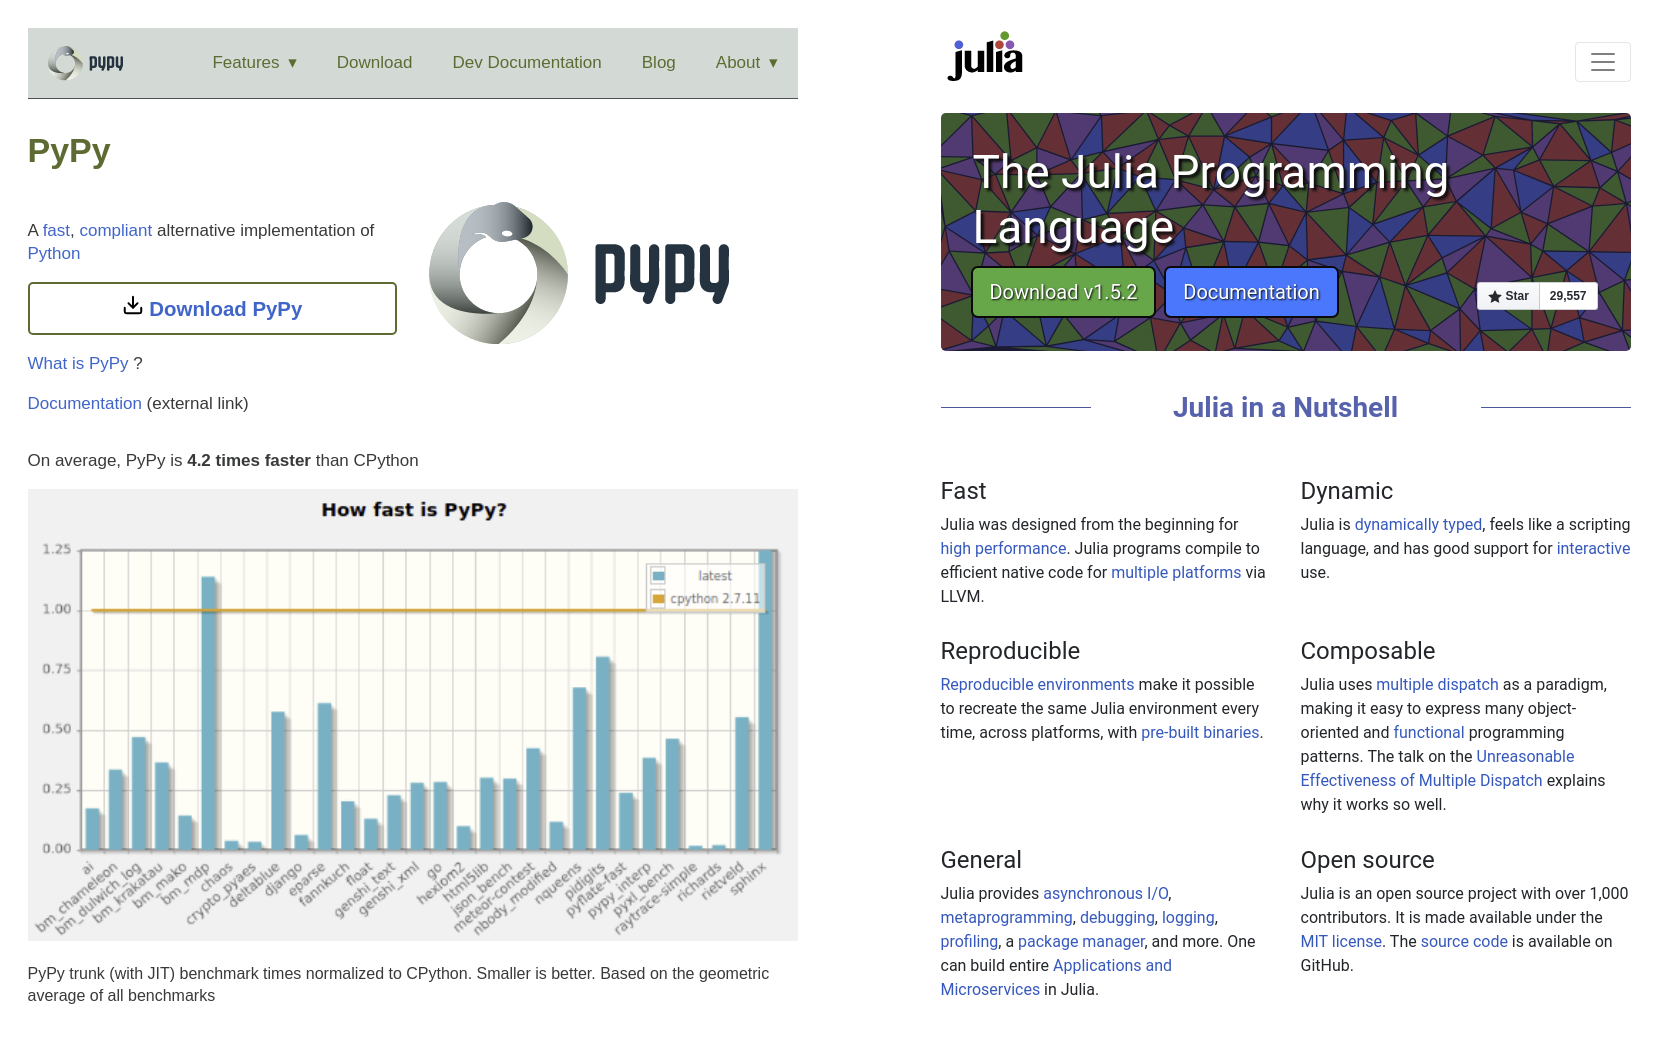
\includegraphics[width=0.91\linewidth]{img/pypy-and-julia.png}
\end{center}
\end{frame}

\begin{frame}{Defining less is good: \textcolor{yellow}{ROOT's RDataFrame} takes away for loops}
\vspace{0.25 cm}

\begin{center}
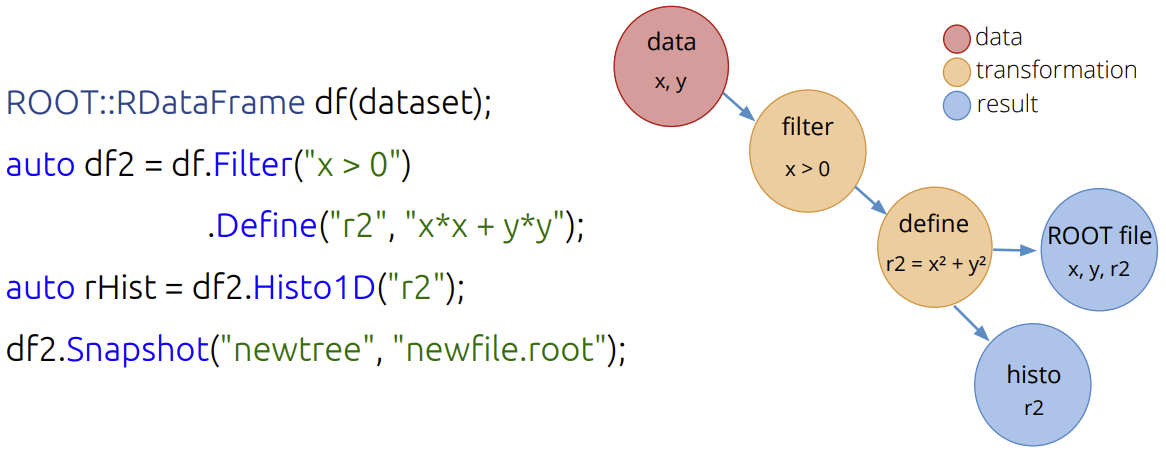
\includegraphics[width=\linewidth]{img/rdataframe-graph.png}
\end{center}

\begin{uncoverenv}<2->
\fbox{\begin{minipage}{\linewidth}
Without an explicit \mintinline{python}{for} loop, tasks without a dependency arrow can be parallelized or distributed across a cluster.
\end{minipage}}
\end{uncoverenv}

\vspace{0.25 cm}
(see Enrico Guiraud @ CHEP 2018)
\end{frame}

\begin{frame}{}
\begin{columns}
\column{1.15\linewidth}
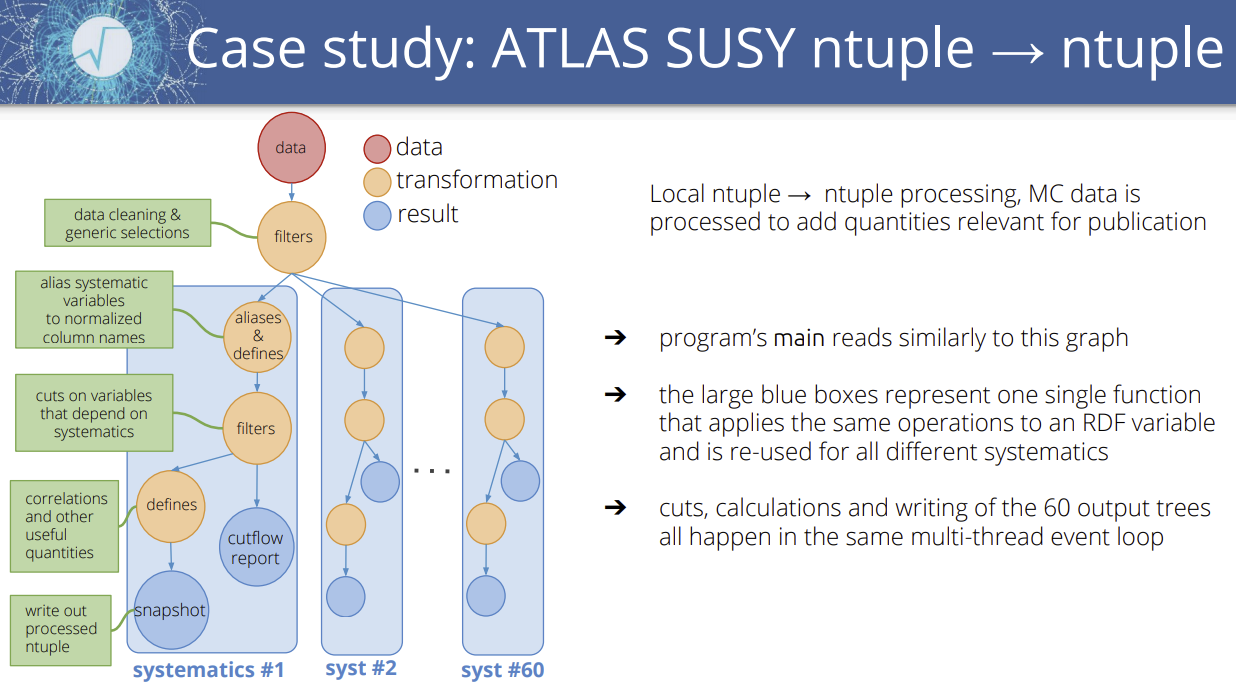
\includegraphics[width=\linewidth]{img/rdataframe-slide-1.png}
\end{columns}
\end{frame}

\begin{frame}{}
\begin{columns}
\column{1.15\linewidth}
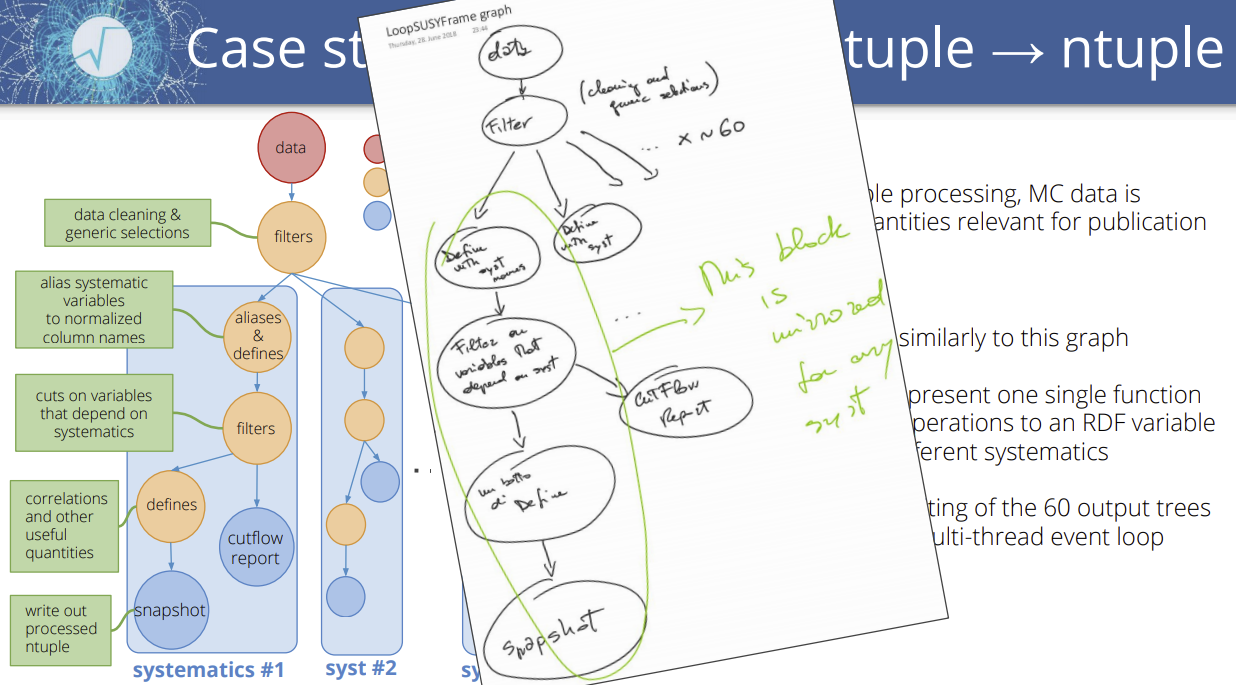
\includegraphics[width=\linewidth]{img/rdataframe-slide-2.png}
\end{columns}
\end{frame}

\begin{frame}{}
\begin{columns}
\column{1.15\linewidth}
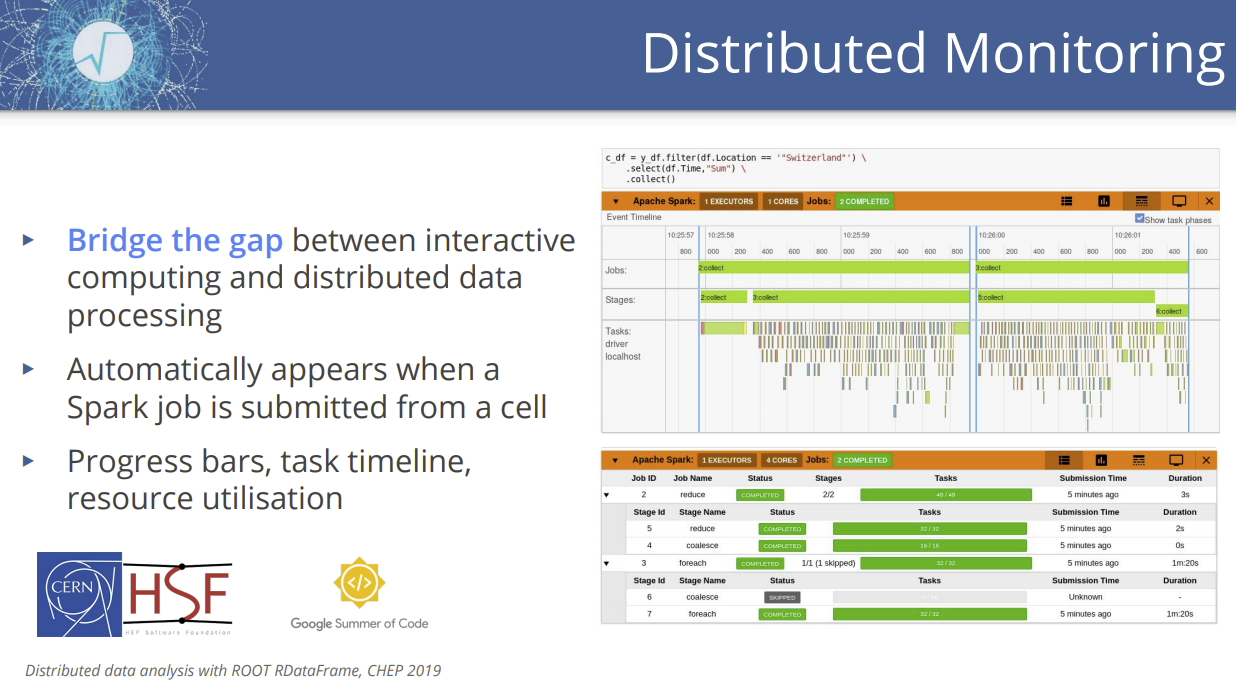
\includegraphics[width=\linewidth]{img/rdataframe-distributed.png}
\end{columns}
\end{frame}

\begin{frame}{RDataFrame also JIT-compiles functions (with Cling)}
\vspace{0.5 cm}

\begin{center}
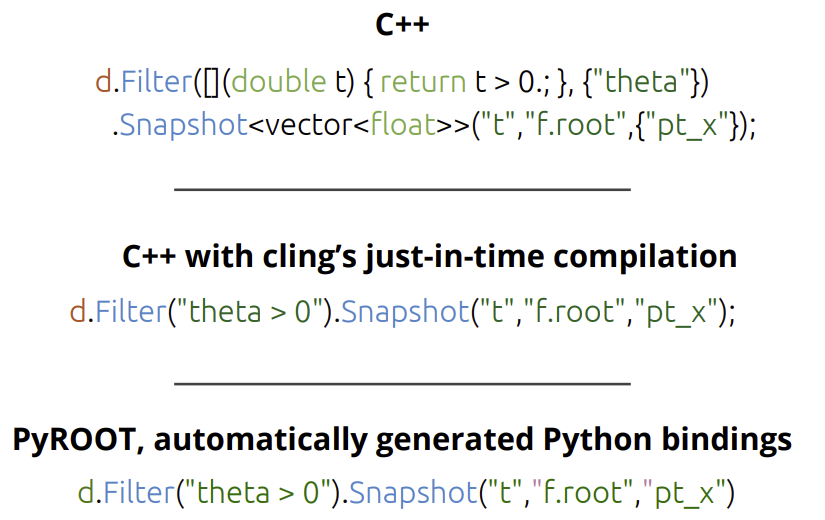
\includegraphics[width=0.7\linewidth]{img/rdataframe-jit.png}
\end{center}
\end{frame}

\begin{frame}[fragile]{Exactly one level of abstraction: \textcolor{yellow}{events}}
\vspace{0.25 cm}
\textcolor{darkblue}{Events are distributed, but event code is C++ on \mbox{\mintinline{c++}{ROOT::VecOps::RVec<Particle>}.\hspace{-1 cm}}}

\scriptsize
\vspace{0.2 cm}
\begin{minted}{python}
getPt_code = """
using namespace ROOT::VecOps;
RVec<double> getPt(const RVec<FourVector> &tracks) {
   auto pt = [](const FourVector &v) { return v.pt(); };
   return Map(tracks, pt);
}
"""
ROOT.gInterpreter.Declare(getPt_code)
\end{minted}
\vspace{0.1 cm}
\begin{minted}{python}
getPtWeights_code = """
using namespace ROOT::VecOps;
RVec<double> getPtWeights(const RVec<FourVector> &tracks) {
   auto ptWeight = [](const FourVector &v) { return 1. / v.Pt(); };
   return Map(tracks, ptWeight);
};
"""
ROOT.gInterpreter.Declare(getPtWeights_code)
\end{minted}
\vspace{0.1 cm}
\begin{minted}{python}
augmented_d = (d.Define("tracks_n", "(int)tracks.size()")
                .Filter("tracks_n > 2")
                .Define("tracks_pts", "getPt(tracks)")
                .Define("tracks_pts_weights", "getPtWeights(tracks)"))
\end{minted}
\end{frame}

\begin{frame}[fragile]{Implicit loops at all levels $\to$ analysis can be completely in Python}
\vspace{0.2 cm}
\hfill \mbox{
\includegraphics[height=1.5 cm]{img/awkward-logo.pdf}\hspace{-0.85 cm}}

\vspace{-1.5 cm}
\scriptsize
\begin{onlyenv}<1>
\begin{minted}{python}
>>> import awkward1 as ak
>>> import numpy as np
>>> 
>>> @ak.mixin_class(ak.behavior)
... class Lorentz:
...     @property
...     def pt(self):
...         return np.sqrt(self.px**2 + self.py**2)
... 
>>> array = ak.Array([{"px": 1, "py": 1, "pz": 1, "E": 1},
...                   {"px": 2, "py": 2, "pz": 2, "E": 2},
...                   {"px": 3, "py": 3, "pz": 3, "E": 3},
...                   {"px": 4, "py": 4, "pz": 4, "E": 4},
...                   {"px": 5, "py": 5, "pz": 5, "E": 5}],
...                  with_name="Lorentz")
... 
\end{minted}
\vspace{3 cm}
\end{onlyenv}
\begin{onlyenv}<2>
\begin{minted}{python}
>>> import awkward1 as ak
>>> import numpy as np
>>> 
>>> @ak.mixin_class(ak.behavior)
... class Lorentz:
...     @property
...     def pt(self):
...         return np.sqrt(self.px**2 + self.py**2)
... 
>>> array = ak.Array([{"px": 1, "py": 1, "pz": 1, "E": 1},
...                   {"px": 2, "py": 2, "pz": 2, "E": 2},
...                   {"px": 3, "py": 3, "pz": 3, "E": 3},
...                   {"px": 4, "py": 4, "pz": 4, "E": 4},
...                   {"px": 5, "py": 5, "pz": 5, "E": 5}],
...                  with_name="Lorentz")
... 
>>> array[-2]
<LorentzRecord {px: 4, py: 4, pz: 4, E: 4} type='Lorentz["px": int64, "py": int6...'>
\end{minted}
\vspace{3 cm}
\end{onlyenv}
\begin{onlyenv}<3>
\begin{minted}{python}
>>> import awkward1 as ak
>>> import numpy as np
>>> 
>>> @ak.mixin_class(ak.behavior)
... class Lorentz:
...     @property
...     def pt(self):
...         return np.sqrt(self.px**2 + self.py**2)
... 
>>> array = ak.Array([{"px": 1, "py": 1, "pz": 1, "E": 1},
...                   {"px": 2, "py": 2, "pz": 2, "E": 2},
...                   {"px": 3, "py": 3, "pz": 3, "E": 3},
...                   {"px": 4, "py": 4, "pz": 4, "E": 4},
...                   {"px": 5, "py": 5, "pz": 5, "E": 5}],
...                  with_name="Lorentz")
... 
>>> array[-2]
<LorentzRecord {px: 4, py: 4, pz: 4, E: 4} type='Lorentz["px": int64, "py": int6...'>
>>> array * 10
<Array [{px: 10, py: 10, pz: 10, ... E: 50}] type='5 * {"px": int64, "py": int64...'>
\end{minted}
\vspace{3 cm}
\end{onlyenv}
\begin{onlyenv}<4>
\begin{minted}{python}
>>> import awkward1 as ak
>>> import numpy as np
>>> 
>>> @ak.mixin_class(ak.behavior)
... class Lorentz:
...     @property
...     def pt(self):
...         return np.sqrt(self.px**2 + self.py**2)
... 
>>> array = ak.Array([{"px": 1, "py": 1, "pz": 1, "E": 1},
...                   {"px": 2, "py": 2, "pz": 2, "E": 2},
...                   {"px": 3, "py": 3, "pz": 3, "E": 3},
...                   {"px": 4, "py": 4, "pz": 4, "E": 4},
...                   {"px": 5, "py": 5, "pz": 5, "E": 5}],
...                  with_name="Lorentz")
... 
>>> array[-2]
<LorentzRecord {px: 4, py: 4, pz: 4, E: 4} type='Lorentz["px": int64, "py": int6...'>
>>> array * 10
<Array [{px: 10, py: 10, pz: 10, ... E: 50}] type='5 * {"px": int64, "py": int64...'>
>>> array.pt
<Array [1.41, 2.83, 4.24, 5.66, 7.07] type='5 * float64'>
\end{minted}
\vspace{3 cm}
\end{onlyenv}
\begin{onlyenv}<5>
\begin{minted}{python}
>>> import awkward1 as ak
>>> import numpy as np
>>> 
>>> @ak.mixin_class(ak.behavior)
... class Lorentz:
...     @property
...     def pt(self):
...         return np.sqrt(self.px**2 + self.py**2)
... 
>>> array = ak.Array([[{"px": 1, "py": 1, "pz": 1, "E": 1},
...                    {"px": 2, "py": 2, "pz": 2, "E": 2},
...                    {"px": 3, "py": 3, "pz": 3, "E": 3}],
...                   [],
...                   [{"px": 4, "py": 4, "pz": 4, "E": 4},
...                    {"px": 5, "py": 5, "pz": 5, "E": 5}]],
...                  with_name="Lorentz")
... 
>>> array[0, -1]
<LorentzRecord {px: 3, py: 3, pz: 3, E: 3} type='Lorentz["px": int64, "py": int6...'>
>>> array * 10
<Array [[{px: 10, py: 10, ... E: 50}]] type='3 * var * {"px": int64, "py": int64...'>
>>> array.pt
<Array [[1.41, 2.83, 4.24], ... [5.66, 7.07]] type='3 * var * float64'>
\end{minted}
\vspace{3 cm}
\end{onlyenv}
\begin{onlyenv}<6>
\begin{minted}{python}
>>> import awkward1 as ak
>>> import numpy as np
>>> 
>>> @ak.mixin_class(ak.behavior)
... class Lorentz:
...     @property
...     def pt(self):
...         return np.sqrt(self.px**2 + self.py**2)
... 
>>> array = ak.Array([[[{"px": 1, "py": 1, "pz": 1, "E": 1},
...                     {"px": 2, "py": 2, "pz": 2, "E": 2}],
...                    [{"px": 3, "py": 3, "pz": 3, "E": 3}]],
...                   [[]],
...                   [[{"px": 4, "py": 4, "pz": 4, "E": 4}],
...                    [],
...                    [{"px": 5, "py": 5, "pz": 5, "E": 5}]]],
...                  with_name="Lorentz")
>>> array[-1, 2, 0]
<LorentzRecord {px: 5, py: 5, pz: 5, E: 5} type='Lorentz["px": int64, "py": int6...'>
>>> array * 10
<Array [[[{px: 10, py: 10, ... E: 50}]]] type='3 * var * var * {"px": int64, "py...'>
>>> array.pt
<Array [[[1.41, 2.83], [4.24, ... [], [7.07]]] type='3 * var * var * float64'>
\end{minted}
\vspace{3 cm}
\end{onlyenv}
\end{frame}

\begin{frame}{Awkward Array is like NumPy, but for data structures}
\vspace{0.2 cm}
\begin{columns}
\column{1.1\linewidth}
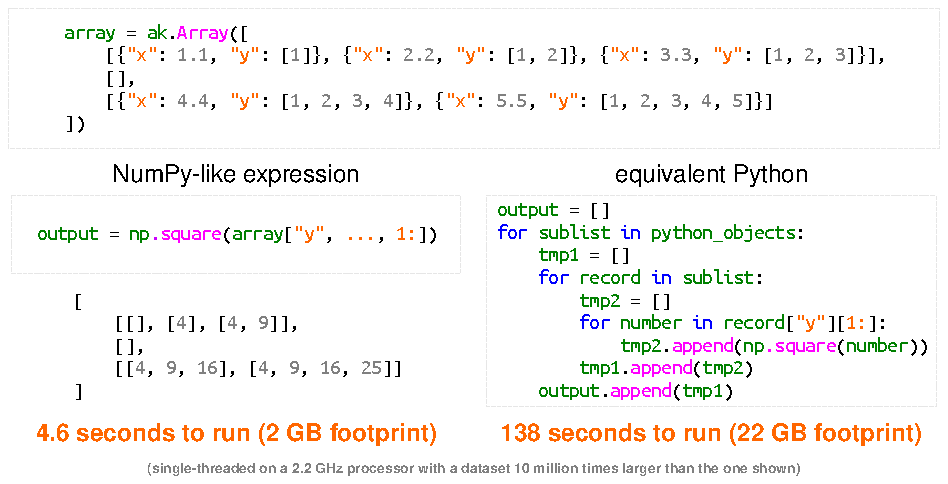
\includegraphics[width=\linewidth]{img/pivarski-one-slide-summary.pdf}
\end{columns}
\end{frame}

\begin{frame}[fragile]{Like NumPy, but structured: \textcolor{yellow}{broadcasting}}
\begin{center}
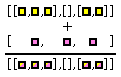
\includegraphics[width=0.4\linewidth]{img/cartoon-broadcasting.pdf}
\end{center}

\begin{columns}
\column{1.03\linewidth}
\begin{minted}{python}
>>> jagged = ak.Array([[1, 2, 3],  [], [4, 5]])
>>> flat   = ak.Array([      100, 200,    300])
>>> jagged + flat
<Array [[101, 102, 103], [], [304, 305]] type='3 * var * int64'>
\end{minted}
\end{columns}
\end{frame}

\begin{frame}[fragile]{Like NumPy, but structured: \textcolor{yellow}{combinatorics}}
\scriptsize
\vspace{0.5 cm}

\begin{columns}
\column{0.5\linewidth}
\textcolor{darkblue}{\Large Cartesian product}

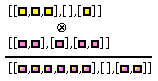
\includegraphics[width=\linewidth]{img/cartoon-cartesian.pdf}

\begin{minted}{python}
>>> x = [[1, 2, 3], [], [4]]
>>> y = [["a", "b"], ["c"], ["d", "e"]]
>>> ak.cartesian([x, y], axis=1)
[[(1, "a"), (1, "b"),
  (2, "a"), (2, "b"),
  (3, "a"), (3, "b")],
 [],
 [(4, "d"), (4, "e")]]
\end{minted}

\column{0.52\linewidth}
\textcolor{darkblue}{\Large Combinations without replacement}

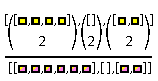
\includegraphics[width=\linewidth]{img/cartoon-combinations.pdf}

\begin{minted}{python}
>>> x = [[1, 2, 3, 4], [], [5, 6]]
>>> ak.combinations(x, 2, axis=1)
[[(1, 2), (1, 3), (1, 4),
  (2, 3), (2, 4), (3, 4)],
 [],
 [(5, 6)]]
\end{minted}
\vspace{\baselineskip}
\end{columns}
\end{frame}

\begin{frame}[fragile]{Like NumPy, but structured: \textcolor{yellow}{reduction}}
\vspace{0.5 cm}

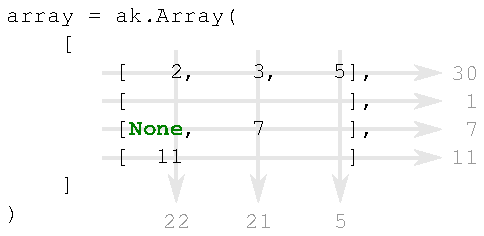
\includegraphics[width=8 cm]{img/reduction.pdf}

\begin{minted}{python}
>>> ak.prod(array, axis=0)
<Array [22, 21, 5] type='3 * int64'>
\end{minted}

\begin{minted}{python}
>>> ak.prod(array, axis=1)
<Array [30, 1, 7, 11] type='4 * int64'>
\end{minted}
\end{frame}

\begin{frame}[fragile]{\textcolor{yellow}{Awkward Arrays} can be used with \textcolor{yellow}{Numba}}
\vspace{0.2 cm}
You can mix fast, explicit \mintinline{python}{for} loops with NumPy-like slicing, all in Python.

\vspace{0.25 cm}
\scriptsize
\begin{minted}{python}
>>> @nb.jit
... def make_cut(electrons, jets, builder):
...     for event_electrons, event_jets in zip(electrons, jets):
...         builder.begin_list()
...         for electron in event_electrons:
...             keep = False
...             for jet in event_jets:
...                 if abs(electron.x - jet.x) < 0.45:   # calculate delta-R here
...                     keep = True
...                     break
...             builder.append(keep)
...         builder.end_list()
...     return builder
... 
>>> cut = make_cut(electrons, jets, ak.ArrayBuilder()).snapshot()
>>> cut
<Array [[True, False, True], ... [True, False]] type='3 * var * bool'>
>>> electrons[cut].tolist()
[[{'x': 1, 'y': 1, 'z': 1, 't': 1}, {'x': 3, 'y': 3, 'z': 3, 't': 3}],
 [],
 [{'x': 4, 'y': 4, 'z': 4, 't': 4}]]
\end{minted}
\end{frame}

\begin{frame}{\textcolor{yellow}{vector}: an Awkward 2D, 3D, Lorentz vector library in development}
\vspace{0.17 cm}
\begin{columns}
\column{1.04\linewidth}
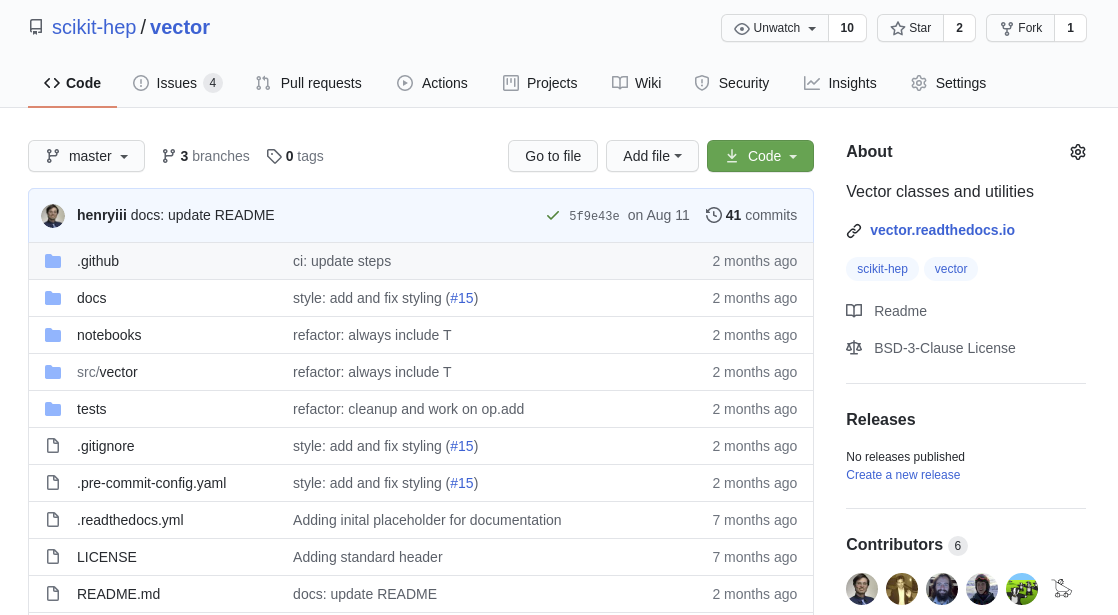
\includegraphics[width=\linewidth]{img/vector-github.png}
\end{columns}
\end{frame}

\begin{frame}{First release of \textcolor{yellow}{hist}, a Pythonic histogram library, on Tuesday}
\vspace{0.18 cm}
\begin{center}
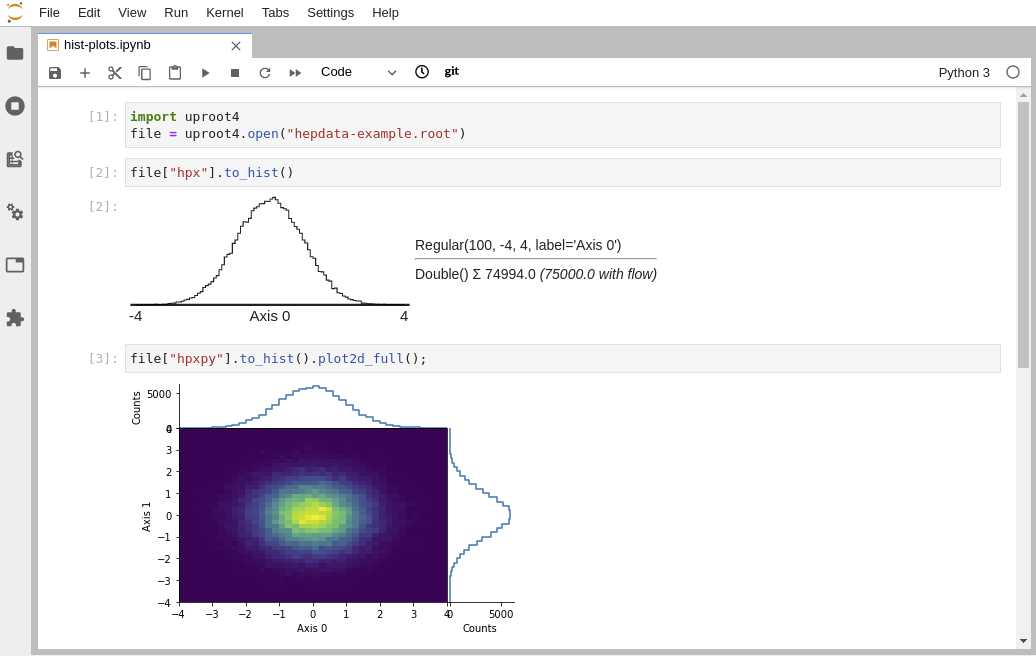
\includegraphics[width=0.85\linewidth]{img/hist-plots.png}
\end{center}
\end{frame}

\begin{frame}{\textcolor{yellow}{hepunits}: common units in HEP and \textcolor{yellow}{particle}: PDG data}
\vspace{0.18 cm}
\begin{center}
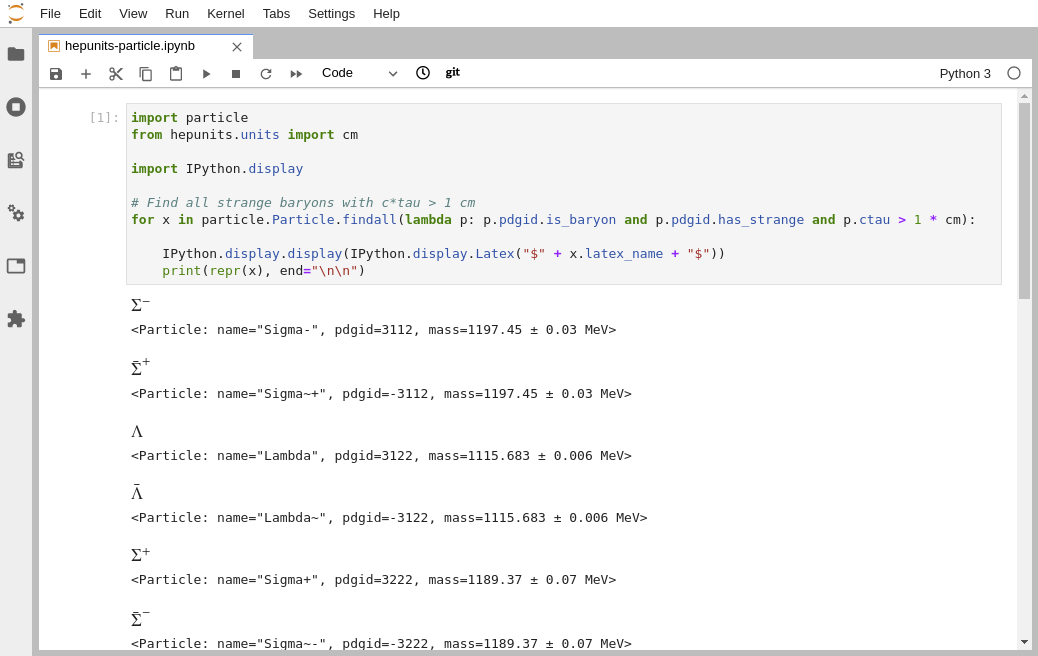
\includegraphics[width=0.85\linewidth]{img/hepunits-particle.png}
\end{center}
\end{frame}

\begin{frame}{\textcolor{yellow}{Scikit-HEP}: a growing ecosystem of interoperating tools}
\vspace{0.15 cm}
\begin{center}

\includegraphics[width=0.85\linewidth]{img/ecosystem.pdf}
\end{center}
\end{frame}

\begin{frame}{\mbox{ }}
\vspace{0.5 cm}

\begin{center}
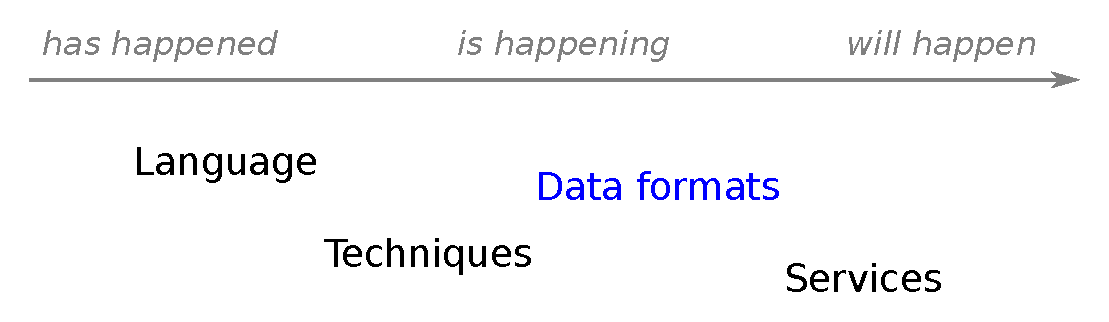
\includegraphics[width=0.9\linewidth]{img/topics-3.pdf}
\end{center}
\end{frame}

\begin{frame}{\mbox{ }}
\vspace{0.5 cm}

\begin{center}
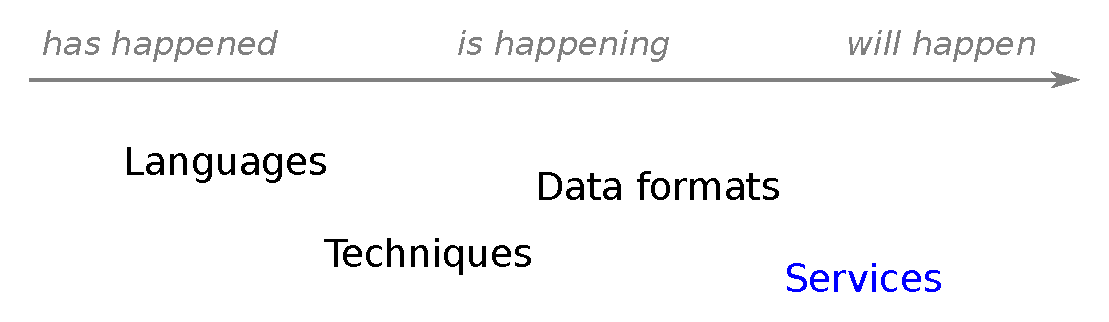
\includegraphics[width=0.9\linewidth]{img/topics-4.pdf}
\end{center}
\end{frame}


\end{document}
